\documentclass[sigplan,screen,nonacm]{acmart}
\settopmatter{printfolios=true}

\usepackage{tikz}
\usetikzlibrary{arrows.meta}
\usepackage{listings}
\lstset{
  basicstyle=\ttfamily\footnotesize,
  breaklines=true,
  frame=single,
  columns=fullflexible,
  keepspaces=true,
}

\title{Rotor in Rust: Fast Generation of RISC-V Machine Models
       with Symbolic Console Arguments}

\author{Jasmin Begi\'{c}}
\affiliation{%
  \institution{Paris Lodron University of Salzburg}
  \city{Salzburg}\country{Austria}}
\email{jask.begic@gmail.com}

\author{Daniel Wassie}
\affiliation{%
  \institution{Paris Lodron University of Salzburg}
  \city{Salzburg}\country{Austria}}
\email{danielkassahun2@gmail.com}

\begin{document}



\begin{abstract}
Rotor generates bit-precise BTOR2 machine models of RISC-V binaries for
bounded model checking. We present a reimplementation of rotor in Rust
that generates the model of selfie's 43k-instruction self-compilation in
0.1 seconds and 20\,MB of memory, where the reference C implementation
requires 139 seconds and 428\,MB --- without doing less work:
counter-based profiling of the subexpression-sharing question in both
tools shows that the difference is one hash probe versus an average of
1.17 million linked-list comparisons per question, 11.7 billion
comparisons in total.
We further extend the generated models with \emph{symbolic console
arguments}, an item the original rotor paper lists as future work: the
bytes of \texttt{argv} are left as uninitialized model states inside an
otherwise concrete process-start stack image, letting the model checker
search over everything a user could type on the command line. On five
test programs whose planted bugs are unreachable through standard input,
the model checker recovers the exact triggering argument bytes within
seconds.
Because a rewrite of a verification tool must itself be validated, we
introduce a differential-testing harness that demands, for every
benchmark, that the same bad-state property becomes satisfiable at the
same minimal bound from both rotors' models. Across the 18 standard
selfie benchmarks under two property configurations --- 36 paired
verdicts --- the two generators are indistinguishable to the model
checker. The harness also exposed a crash in the reference
implementation and, once, a bug in our own measurement infrastructure.
Finally, an interactive browser-based visualizer replays counterexample
witnesses step by step, completing the pipeline from binary to
human-readable verification result.
\end{abstract}

\keywords{bounded model checking, BTOR2, RISC-V, symbolic execution,
differential testing, Rust}

\maketitle

\section{Introduction}

Bounded model checking (BMC)~\cite{biere1999} decides whether a system
can reach a bad state within a fixed number of execution steps --- for
\emph{any} input. Applied to software at the machine-code level, BMC
offers an attractive guarantee: what is verified is the binary that
actually runs, not a source-level abstraction of it. The rotor
tool~\cite{rotorpaper}, part of the selfie project~\cite{selfie}, makes
this workflow concrete: it translates a RISC-V~\cite{riscv} binary into
a BTOR2~\cite{btor2} model --- a bit-precise description of a machine
executing that binary --- which bounded model checkers such as
\texttt{btormc} check against safety properties like division by zero,
segmentation faults, and reaching a target exit code.

In practice, three obstacles limit who can use this pipeline, what bugs
it can find, and what a user can do with the answer.

First, the reference rotor is a single 14{,}000-line
C\textsuperscript{*} file. Beyond the engineering cost of extending it,
it is slow on large inputs: generating the model of selfie's
self-compilation takes over two minutes and hundreds of megabytes of
memory, which makes regenerate-after-every-change workflows impractical.

Second, the generated models expose only one input surface to the model
checker: bytes read from standard input. Programs also receive input
through \emph{console arguments}, and bugs that depend on a specific
argument are structurally invisible --- the model fixes the argument
bytes, so no solver, however powerful, may explore them. The rotor paper
itself names ``console arguments as symbolic input'' as future
work~\cite{rotorpaper}.

Third, when the model checker does find a counterexample, its witness is
a flat list of binary-encoded assignments keyed to internal node numbers
--- sound, complete, and unreadable for anyone who did not build the
tool.

This paper addresses all three obstacles. We reimplement rotor as a
modular Rust crate; we extend the machine models with symbolic console
arguments; and we provide an interactive visualizer for witnesses. A
rewrite of a verification tool, however, raises an obligation that
ordinary software does not: the new tool's claim to correctness must
itself be checkable. We therefore make the validation methodology a
contribution in its own right: a differential-testing harness that
treats the model checker as an impartial referee between the two
generators, with a criterion strict enough that every modeling defect we
introduced during development was caught by it.

\medskip
\noindent\textbf{Contributions.} To summarise:
\begin{itemize}
  \item A modular Rust reimplementation of rotor that emits the same 24
        bad-state properties as the reference, generates models three
        orders of magnitude faster in $21\times$ less memory, and
        supports the full pipeline from ELF binary to BTOR2 model
        (Section~\ref{sec:rust}).
  \item Symbolic console arguments: \texttt{argv} content bytes become
        uninitialized model states inside an otherwise concrete
        process-start stack image, conservatively extending the machine
        input of the original models (Section~\ref{sec:argv}).
  \item A differential-validation methodology and harness: same
        bad-state property at the same minimal bound, demanded across
        the full benchmark suite under multiple configurations; 36/36
        paired verdicts agree (Section~\ref{sec:validation}).
  \item A counter-based performance analysis, following classical
        profiling methodology, that fully attributes the performance
        difference between the two generators and uncovers an
        architectural difference in \emph{when} each tool deduplicates
        (Section~\ref{sec:performance}); we close the argument by porting
        the optimisation \emph{back into the reference C}, where it is
        $\sim$95$\times$ faster with byte-identical output
        (Section~\ref{sec:backport}).
  \item An interactive, browser-based witness visualizer
        (Section~\ref{sec:visualizer}).
\end{itemize}

\noindent\textbf{Artifacts.} All artifacts are public: the Rust
implementation, the validation harness with both result tables, the C
reference models with their generation commands recorded in file
headers, a reproducible Docker setup for the model checker and for the
crash described in Section~\ref{sec:cse}, the hash-consing back-port of
the reference C (full source, unified diffs, and its own differential
validation), and the visualizer with twelve preloaded examples:
\begin{center}
\footnotesize
\url{https://github.com/jaspek/rotor-rust}\\
\url{https://github.com/jaspek/rotor-c-hashcons}\\
\url{https://jaspek.github.io/rotor-rust/}
\end{center}

\section{Background}
\label{sec:background}

\subsection{Rotor models}

A rotor-generated BTOR2 model describes a RISC-V machine as a transition
system: \emph{states} (program counter, 32 general-purpose registers,
byte- or word-addressed arrays for the code, data, heap, and stack
segments, and kernel state such as the program break and input
counters), \emph{transition functions} giving each state's next value as
a function of the current state --- the semantics of every instruction
the binary contains --- and \emph{bad-state properties}, boolean
formulas over the state that encode safety violations. The reference
emits 24 properties, among them division by zero, signed division
overflow, illegal and unknown instructions, fetch/load/store address
validity and segmentation faults, stack-pointer validity, unknown
system calls, argument faults of the modeled system calls, and reaching
a configurable target exit code.

Machine input enters the model through \emph{uninitialized} states:
BTOR2 states without an \texttt{init} assignment may take any value of
their sort in the initial state, so the model checker quantifies over
them. The reference models a bounded standard-input buffer this way. A
bounded model checker unrolls the transition system and asks, for
increasing $k$, whether some assignment of the uninitialized states
reaches a bad state within $k$ steps; \texttt{btormc} reports the
property index and the minimal such $k$, together with a witness.

The rotor paper establishes that its models are \emph{sound and
complete at bit level}: a machine state is reachable on a RISC-V
machine within $k$ instructions for some input exactly when the model
is $k$-satisfiable for that input~\cite{rotorpaper}. This property is
what gives our comparison its leverage. Because each model is a
faithful mirror of a machine, two models of the \emph{same} binary that
disagree --- on which property fires, or after how many transitions ---
mirror two \emph{different} machines; conversely, if no disagreement
can be exhibited, the machines coincide on everything the solver can
observe. Our validation (Section~\ref{sec:validation}) is the
systematic search for such a disagreement.

\subsection{The BTOR2 format by example}
\label{sec:btor2}

BTOR2 is a line-oriented format: every line introduces a node with a
numeric id, and later lines refer to earlier ones by id. The following
complete model counts upward by a machine-chosen step and asks whether
the counter can reach 200:

\begin{lstlisting}
1  sort bitvec 1        ; Boolean
2  sort bitvec 8        ; a byte
3  constd 2 0
4  state 2 counter
5  init 2 4 3           ; counter := 0
6  state 2 delta        ; NO init: model input
7  add 2 4 6
8  next 2 4 7           ; counter' = counter+delta
9  constd 2 200
10 ugte 1 4 9
11 bad 10 counter-overflow
\end{lstlisting}

\noindent Line 6 is the whole input mechanism: a state without an
\texttt{init} may take any value of its sort in the initial state, and
--- because it also has no \texttt{next} --- may be re-chosen at every
step. The model checker therefore quantifies over all sequences of
\texttt{delta} values; \texttt{btormc} answers that the bad state is
reachable at bound $k{=}1$ (choose $\texttt{delta} \geq 200$
immediately). When an input must stay \emph{fixed} after the initial
state --- a file's contents, a command-line argument --- the generator
adds a self-loop \texttt{next}, freezing the nondeterministic choice at
step zero. Both devices appear throughout rotor models and both matter
in Section~\ref{sec:argv}.

A rotor model of a real binary is this same skeleton at scale: tens of
registers and memory arrays instead of one counter, one transition
function per state built from the semantics of every instruction in the
binary, and 24 \texttt{bad} lines instead of one.

\subsection{A worked example}
\label{sec:worked}

Consider \texttt{division-by-zero-3-35.c} from the benchmark suite. The
program allocates one machine word on the heap, reads one byte of input
into it, subtracts 48, and divides a constant by the result --- so the
input byte \texttt{'0'} (ASCII 48) makes the divisor zero. Rotor
compiles nothing and executes nothing; it emits a model whose initial
state is the loaded binary with the boot stack image, whose transition
functions encode selfie's startup code, the \texttt{malloc}/\texttt{brk}
round trip, the stalling \texttt{read}, and the arithmetic, and whose
property b7 is
\begin{lstlisting}
40901 eq 1 20055 50 ; actual exit code ==
                    ; bad exit code?
\end{lstlisting}
\noindent style boolean logic over the state (here shown for the exit
property; the division property guards the divisor of every division
instruction in the binary). Running \texttt{btormc} on the model yields
\begin{lstlisting}
[btor>mc] bad state property 7 reachable
          at bound k = 76 SATISFIABLE
\end{lstlisting}
\noindent meaning: of all 256 possible input bytes, at least one ---
the witness shows \texttt{0x30} $=$ \texttt{'0'} --- drives the machine
into the division-by-zero bad state, and the earliest this can happen
is after exactly 76 machine transitions, counting every startup
instruction, the system-call round trips, and the byte delivery of the
stalling \texttt{read}. This pair, (property index, minimal bound), is
the unit of comparison throughout this paper.

\subsection{The benchmark suite}

The rotor paper's experiments use 18 small C\textsuperscript{*} programs
(selfie's \texttt{examples/symbolic}), each reading one byte of input,
with planted bugs that fire between 66 and 1438 unrolling
steps~\cite{rotorpaper}. We adopt the same suite, the same single input
byte, and the same machine configuration (64-bit words, 32-bit virtual
address space, 2048-byte heap and stack allowances) throughout.

\section{Rotor in Rust}
\label{sec:rust}

\subsection{Architecture}

The reimplementation is a Rust crate organised by concern: a BTOR2
\emph{builder} (typed node graph, hash-consing, printing), a
\emph{machine} layer (sorts, register file, segmented memory, kernel
state), a RISC-V \emph{decoder} (RV64/RV32 base, M and C extensions,
ELF loading), and a \emph{model} layer (per-instruction data flow,
sequential next-state logic, the 24 properties). Each BTOR2 node is a
value of a typed \texttt{enum}; structurally equal nodes are interned
through a hash map at creation:

\begin{lstlisting}
fn intern(&mut self, op: Op, ...) -> NodeId {
  self.profile_lookups += 1;
  if self.enable_cse {
    if let Some(&id) = self.dedup.get(&op) {
      self.profile_hits += 1;
      return id;          // duplicate: never allocated
    }
  }
  let id = self.alloc_id();
  self.nodes.push(Node { id, op: op.clone(), .. });
  if self.enable_cse { self.dedup.insert(op, id); }
  id
}
\end{lstlisting}

\noindent Because the probe precedes allocation, a duplicate or dead
node is never created. This single data-structure decision dominates
the performance comparison in Section~\ref{sec:performance}; the
\texttt{profile\_*} counters appear in
Section~\ref{sec:performance} as well. The same builder serves a
\texttt{--no-cse} mode (Section~\ref{sec:cse}) and a comment-stripping
mode mirroring the reference's \texttt{-nocomments}, both used in the
evaluation. Table~\ref{tab:modules} summarises the crate layout.

\begin{table}[t]
\caption{Crate layout: one module per concern.}
\label{tab:modules}
\centering
\footnotesize
\begin{tabular}{ll}
\toprule
Module & Responsibility \\
\midrule
\texttt{btor2/builder} & node interning (hash-consing), id allocation \\
\texttt{btor2/node, sort} & typed \texttt{Op} enum; bit-vector/array sorts \\
\texttt{btor2/printer} & text output in creation order \\
\texttt{riscv/elf\_loader} & ELF segments via \texttt{goblin} \\
\texttt{riscv/decode, compressed} & RV64/RV32 base, M, C decoding \\
\texttt{machine/sorts, registers} & machine sorts, register file \\
\texttt{machine/memory, segmentation} & segment arrays, bounds logic \\
\texttt{machine/kernel} & break, file descriptor, input counters \\
\texttt{model/combinational} & per-instruction data flow \\
\texttt{model/sequential} & next-state functions \\
\texttt{model/properties} & the 24 bad states, in reference order \\
\texttt{model/generator} & four-phase pipeline, CLI surface \\
\bottomrule
\end{tabular}
\end{table}

\emph{Determinism.} Generation is fully deterministic: nodes are printed
in creation order, no hash-map iteration reaches the output path, and no
randomness exists anywhere in the generator. The same binary and flags
therefore produce byte-identical models across runs \emph{and across
platforms} --- our continuous integration exploits this by regenerating
all 18 benchmark models on every push (on Linux, from models originally
verified on Windows) and requiring the division model to compare equal,
byte for byte, against the committed artifact of the validation
campaign. Reproducibility is thus not a promise but a gate the
repository enforces on itself.

\subsection{Faithfulness requirements}
\label{sec:faithful}

Emitting the same properties is not sufficient for two generators to
agree; the modeled \emph{machines} must be identical. Differential
validation (Section~\ref{sec:validation}) forced us to reproduce, item
by item, semantics that are easy to get subtly wrong:

\begin{itemize}
  \item \emph{Deterministic initial memory.} All segment arrays and the
        register file are zero-initialized before the binary image is
        written. An uninitialized array would let the solver invent
        memory contents and produce spurious counterexamples.
  \item \emph{Exact segment geometry.} The heap begins at the first
        page-aligned address after the data segment; the stack occupies
        $[2^{32}{-}\textit{allowance},\,2^{32})$ with its end wrapped to
        zero in the 32-bit virtual address sort, requiring wrap-aware
        bounds checks; the program break starts at the heap start.
  \item \emph{Process-start stack image.} The stack is initialized with
        a concrete \texttt{argc}/\texttt{argv} image --- argument count,
        pointer array, terminating null pointers, and the program-name
        string --- exactly as selfie's boot loader writes it.
  \item \emph{System-call semantics.} The \texttt{read} system call
        delivers \emph{one input byte per machine transition} with the
        program counter stalled until the read completes; \texttt{exit}
        stalls the machine forever; \texttt{brk} validates the requested
        break against the heap segment; \texttt{openat} maintains a
        file-descriptor counter.
  \item \emph{Property emission order.} The 24 properties are emitted in
        the reference's exact order, so that \texttt{btormc} property
        \emph{indices} are comparable across both models.
\end{itemize}

The geometry items are directly checkable against the reference's
output, because the reference prints its segment boundaries as named
constants. For the worked example the reference model contains
\begin{lstlisting}
consth 4 00010000 ; start of code segment
consth 4 00011008 ; end of data segment
consth 4 00012000 ; start of heap segment
consth 4 FFFFF800 ; start of stack segment
consth 4 00000000 ; end of stack segment
\end{lstlisting}
\noindent --- note the heap starting at the page boundary
\texttt{0x12000} rather than at the data end \texttt{0x11008}, and the
stack end printed as \emph{zero}: $2^{32}$ does not fit in the 32-bit
virtual-address sort, so the constant wraps, and every upper-bound
comparison against it must be skipped rather than evaluated. Our first
implementation aligned the heap to nothing and compared against the
wrapped zero; both mistakes produce models that are subtly, detectably
different machines.

Each property body was ported from the reference source rather than
re-derived, and the porting process itself illustrates why this
discipline matters. Three of our initial, plausible-looking
formulations differed from the reference. We had assumed the
break-validity check requires the new program break to be at least the
current one; the reference checks only the upper bound, so that
\texttt{brk(0)} address queries --- which selfie's startup performs ---
are valid, and our version fired a spurious fault at bound 5. We had
checked the \texttt{openat} filename as a single address; the reference
checks the full range $[\mathit{a1}, \mathit{a1}+127]$ against the heap
segment. And we had checked the \texttt{read} buffer on every
transition of an ongoing read; the reference checks it once, when the
read starts. All three differences were exposed by the validation
harness (Section~\ref{sec:validation}) before they could do harm ---
and none of them would have been caught by reviewing the properties'
names or by comparing model sizes.

Property emission order matters for a subtle practical reason: before
we aligned it, both rotors agreed that division-by-zero is reachable at
bound 76 on the worked example, but reported it as property b1 versus
b7 --- the same property under different indices. Aligning the order
makes the model checker's raw output directly comparable, with no
mapping layer that could itself harbor bugs.

\section{Symbolic Console Arguments}
\label{sec:argv}

\subsection{Mechanism}

At process start, the operating system writes the argument strings, an
array of pointers to them, and the argument count onto the stack. With
\texttt{--symbolic-argv}, our generator builds exactly this layout, but
emits the \emph{content bytes} of \texttt{argv[1..N]} as uninitialized
one-byte states --- the same formal device the reference already uses
for standard input. Everything else remains concrete: \texttt{argc},
all pointers, the terminating null bytes of each string, and
\texttt{argv[0]}. The modeled program reads its arguments through
ordinary loads; the decoder, memory model, and properties are untouched.
Soundness is inherited from the underlying framework: a witness
assignment of the argument bytes corresponds to a real command line,
and conversely every command line within the configured bounds is an
admissible assignment.

The stack image, from the top of memory downward, consists of the
string area (for each symbolic argument, \texttt{max\_arglen} symbolic
bytes followed by a concrete null terminator; \texttt{argv[0]} is the
concrete program name), the pointer area (\texttt{argv[0..N]} addresses
followed by a null pointer), and \texttt{argc} at the initial stack
pointer --- the standard process-start convention. The symbolic bytes
are additionally frozen with a self-loop \texttt{next}, mirroring how
the reference freezes its input buffer: a state without a \texttt{next}
may be re-chosen by the solver at every step, whereas a command-line
argument is fixed once at process start.

\begin{figure}[t]
\centering
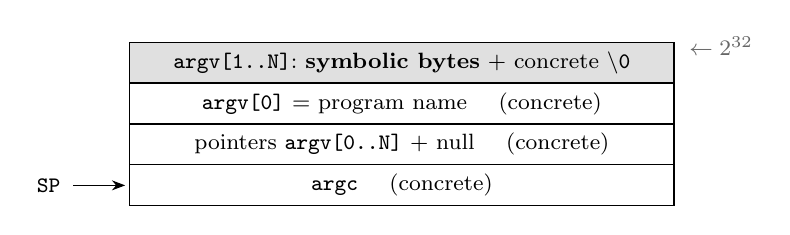
\begin{tikzpicture}[yscale=0.52, xscale=0.72, font=\footnotesize]
  \fill[black!12] (0,3) rectangle (9.6,4);
  \draw (0,3) rectangle (9.6,4);
  \node at (4.8,3.5)
    {\texttt{argv[1..N]}: \textbf{symbolic bytes} + concrete \texttt{\textbackslash0}};
  \draw (0,2) rectangle (9.6,3);
  \node at (4.8,2.5) {\texttt{argv[0]} = program name \quad (concrete)};
  \draw (0,1) rectangle (9.6,2);
  \node at (4.8,1.5) {pointers \texttt{argv[0..N]} + null \quad (concrete)};
  \draw (0,0) rectangle (9.6,1);
  \node at (4.8,0.5) {\texttt{argc} \quad (concrete)};
  \draw[-{Stealth}] (-1.0,0.5) -- (-0.08,0.5);
  \node[anchor=east] at (-1.05,0.5) {\texttt{SP}};
  \node[anchor=west, black!60] at (9.7,3.9) {$\leftarrow 2^{32}$};
\end{tikzpicture}
\caption{The process-start stack image under
\texttt{--symbolic-argv}. Only the shaded argument bytes are open to
the solver; layout, count, pointers, and terminators are concrete.}
\label{fig:stack}
\end{figure}

Figure~\ref{fig:stack} shows the resulting initial stack.
Realizability deserves care in both directions. \emph{Witness to
world:} a satisfying assignment gives each argument byte a concrete
value; the corresponding real command line is the one whose argument
strings contain exactly those bytes up to each string's first zero
byte, so every witness is executable. \emph{World to witness:} any real
invocation whose arguments fit the configured count and length bounds
corresponds to an admissible assignment, so no bug within those bounds
is missed. The bounds themselves are the same compromise the reference
already makes for standard input, whose buffer is likewise finite; and
they are visible, not hidden --- both appear as explicit constants in
the generated model's header comments.

Three design choices keep the model finite and static. \emph{(i)}~The
argument count is fixed at generation time
(\texttt{--num-symbolic-args}); the solver explores argument
\emph{content}, not count. \emph{(ii)}~Each argument occupies a
fixed-size slot of \texttt{--max-arglen} bytes plus a concrete
terminator, bounding input like the reference bounds its input buffer.
\emph{(iii)}~Interior zero bytes are permitted and correspond to shorter
real-world strings. The fixed-slot layout differs from the packed layout
of a real \texttt{execve} only for programs that walk pointers past a
string terminator; for programs treating arguments as C strings the two
are indistinguishable.

\subsection{Validation programs}
\label{sec:argvtests}

We wrote five C\textsuperscript{*} programs whose planted bugs depend
only on console arguments; none reads standard input, so none of these
bugs is expressible in the original models at all
(Table~\ref{tab:argv}).

\begin{table}[t]
\caption{Argv test programs. The bug (\texttt{return 1}) fires iff the
condition holds; the model checker must synthesise the bytes.}
\label{tab:argv}
\centering
\footnotesize
\begin{tabular}{lllr}
\toprule
Test & Bug condition & Class & $k$ \\
\midrule
1 & \texttt{argv[1][0]} $=$ 67 (\texttt{'C'}) & exact byte & 67 \\
2 & $\texttt{argv[1][0]}{\cdot}256 + \texttt{argv[1][1]} = 16706$ & ordered pair & 86 \\
3 & \texttt{argv[1][0]} $\neq 0 \wedge$ \texttt{argv[1][1]} $= 0$ & length & 84 \\
4 & \texttt{argv[1][0]}$=$\texttt{'X'} $\wedge$ \texttt{argv[2][0]}$=$\texttt{'Y'} & two args & 91 \\
5 & \texttt{argv[1][0]} $+$ \texttt{argv[1][1]} $= 200$ & arithmetic & 83 \\
\bottomrule
\end{tabular}
\end{table}

On every program, \texttt{btormc} finds the planted bug within seconds;
the measured minimal bounds appear in the table's last column, and the
witnesses --- committed alongside the models as visualizer examples ---
contain exactly the designed bytes. For test~1 the bad-exit-code
property becomes satisfiable at bound $k{=}67$ with witness byte
\texttt{argv[1][0]} $=$ \texttt{0x43} $=$ \texttt{'C'} --- a value the
solver reaches through three pointer dereferences of the modeled stack
image: from the stack cell at \texttt{SP{+}8} to the pointer array, to
the string slot, to the byte the program's arithmetic actually
inspects. The witness's opening lines are literal enough to quote:
\begin{lstlisting}
sat
b23
#0
3 01000011 argv[1][0]#0
\end{lstlisting}
\noindent --- property \texttt{b23} (the target exit code) is
satisfiable, and the solver's chosen value for the first symbolic
argument byte is \texttt{01000011}, which is 67, which is \texttt{'C'}.
The remaining argument bytes are unconstrained in the witness, exactly
as they should be: the program never reads them, so no value of theirs
can matter. The spread of bounds is itself informative: test~4, which
constrains two \emph{different} arguments simultaneously, needs the
longest path (91 transitions) because the program walks both argument
pointers; no exploration of standard input could produce its bug at any
depth, since the model without symbolic arguments fixes both bytes to
zero.

\section{Differential Validation}
\label{sec:validation}

\subsection{Criterion}

Textual comparison of the generated files is meaningless --- the two
tools serialize the same content differently
(Section~\ref{sec:size}) --- and formal equivalence of the two
generators is out of reach; the rotor paper lists formal verification
of rotor itself as future work~\cite{rotorpaper}. Our criterion is
behavioural and uses the model checker as an impartial referee, in the
spirit of differential testing~\cite{mckeeman}:

\begin{quote}
For the same binary and identical generation parameters, both models
must make the \emph{same property index} satisfiable at the \emph{same
minimal bound} $k$ --- or both must remain unsatisfiable through the
bound limit.
\end{quote}

Stated precisely: let $V(M) \in (\{b_0,\dots,b_{23}\} \times
\mathbb{N}) \cup \{\textsc{unsat}\}$ be the model checker's verdict on
model $M$ --- the least $k \le k_{\max}$ at which some property is
satisfiable, together with that property's index, or \textsc{unsat} if
none is. Two generators \emph{agree on a binary} $B$ under parameters
$\theta$ iff $V(\mathit{gen}_C(B,\theta)) =
V(\mathit{gen}_{\mathit{Rust}}(B,\theta))$, and the campaign demands
agreement for every benchmark under every tested $\theta$.

The criterion is strict because $k$ counts every machine transition on
the violating path, from the boot state to the violation: a single
extra or missing instruction anywhere --- in the boot image, an
instruction's semantics, a system call --- shifts $k$ or changes the
property. The verdict also quantifies over all inputs, so no difference
can hide behind input choice. It is also \emph{transitive} in a useful
way: Section~\ref{sec:backport} reuses the identical criterion, with
the roles recast, to certify a modification of the reference against
the unmodified reference.

\subsection{Setup}

For each of the 18 benchmarks we generate the reference model with the
unmodified C rotor (the generation command is recorded in each output
file's header) and our model with matching parameters, validate both
with \texttt{catbtor} and a $k{=}0$ \texttt{btormc} load, then run
\texttt{btormc} with $k_{\max} = 1500$, which covers the bound range the
rotor paper reports (66--1438). The harness records the (property, $k$)
pair or UNSAT per side and compares; benchmark/rotor pairs run as
isolated containers, parallelised across cores.

\emph{Provenance.} Every claim about ``the reference's model'' is
checkable from the artifact itself: the C rotor records its own
invocation and full parameter set in each output file's header
comments, so the committed reference models carry the proof that they
were produced by the unmodified tool under the stated flags. The
checking toolchain is likewise pinned --- \texttt{catbtor} and
\texttt{btormc} are built from the official Boolector repositories
inside a committed Dockerfile --- so the entire experiment reproduces
from the repository with no unstated dependencies.

\subsection{Results}

\begin{table}[t]
\caption{Differential validation, target exit code 0. Both rotors'
verdicts are identical on every row ($k_{\max}{=}1500$).}
\label{tab:equiv}
\centering
\footnotesize
\begin{tabular}{lll}
\toprule
Benchmark & Property (both) & $k$ (both) \\
\midrule
division-by-zero-3-35 & division-by-zero & 76 \\
invalid-memory-access-fail-2-35 & store-invalid-address & 79 \\
memory-access-fail-1-35 & load-seg-fault & 66 \\
nested-if-else-1-35 & bad-exit-code & 100 \\
nested-if-else-reverse-1-35 & bad-exit-code & 103 \\
nested-recursion-fail-1-35 & --- & UNSAT \\
recursive-ackermann-1-35 & bad-exit-code & 152 \\
recursive-factorial-fail-1-35 & bad-exit-code & 119 \\
recursive-fibonacci-1-10 & bad-exit-code & 118 \\
return-from-loop-1-35 & --- & UNSAT \\
simple-assignment-1-35 & bad-exit-code & 96 \\
simple-decreasing-loop-1-35 & bad-exit-code & 99 \\
simple-if-else-1-35 & bad-exit-code & 108 \\
simple-if-else-reverse-1-35 & bad-exit-code & 108 \\
simple-if-without-else-1-35 & bad-exit-code & 101 \\
simple-increasing-loop-1-35 & bad-exit-code & 93 \\
three-level-nested-loop-fail-1-35 & bad-exit-code & 103 \\
two-level-nested-loop-1-35 & bad-exit-code & 99 \\
\bottomrule
\end{tabular}
\end{table}

Table~\ref{tab:equiv} shows the first configuration (target exit code
0): 16 benchmarks satisfiable with identical property and identical
minimal bound --- five distinct property types, including recursion
matched step-exactly through 152 transitions of nested call frames ---
and two agreed-UNSAT rows.

\begin{table}[t]
\caption{Differential validation, target exit code 1 (the planted
``non-zero exit code'' bugs of the original experiments). Again
identical on every row.}
\label{tab:equiv1}
\centering
\footnotesize
\begin{tabular}{lll}
\toprule
Benchmark group & Property (both) & $k$ (both) \\
\midrule
division-by-zero-3-35 & division-by-zero & 76 \\
invalid-memory-access-fail-2-35 & store-invalid-address & 79 \\
memory-access-fail-1-35 & load-seg-fault & 66 \\
return-from-loop-1-35 & bad-exit-code & 95 \\
simple-assignment-1-35 & bad-exit-code & 91 \\
simple-if-else-1-35 & bad-exit-code & 107 \\
simple-if-else-reverse-1-35 & bad-exit-code & 105 \\
simple-if-without-else-1-35 & bad-exit-code & 106 \\
remaining ten benchmarks & --- & UNSAT \\
\bottomrule
\end{tabular}
\end{table}

A second configuration targeting exit code 1 --- the planted
``non-zero exit code'' bugs of the original
experiments~\cite{rotorpaper}, with the reference models regenerated by
the unmodified C rotor under \texttt{-~1} --- again agrees on all 18
(Table~\ref{tab:equiv1}): the three exit-independent properties fire at
unchanged bounds (they precede any exit on their violating paths), five
planted bugs fire at $k \in [91,107]$ with identical $k$, and the
remaining ten are UNSAT on both sides. Notably,
\texttt{return-from-loop} \emph{flips} from UNSAT to satisfiable at
$k{=}95$ between the configurations --- identically in both rotors ---
so the agreement is not an artifact of one parameter choice, and the
configuration change exercises genuinely different behaviour. In total:
36 paired verdicts, zero divergences. Our lowest observed bound, 66,
equals the lowest bound reported in the rotor paper.

\subsection{A cautionary baseline}
\label{sec:vacuous}

Our first comparison, before this methodology existed, ran both models
at $k_{\max}{=}35$ and found the two rotors ``agreeing'' on all 18
benchmarks. The agreement was vacuous: no property of any benchmark
fires before bound 66, so both sides reported UNSAT everywhere and the
test could not have failed. Worse, the models at that time were
\emph{not} equivalent --- the defects of Section~\ref{sec:faithful}
were all present and undetected. A differential criterion is only as
strong as the depth it explores; calibrating $k_{\max}$ against
known-positive bounds (here, the 66--1438 range the rotor paper
publishes) is what turned the harness from a formality into an
instrument. We report this because the failure mode is silent and, we
suspect, common.

\subsection{Harness engineering}
\label{sec:harness}

Four engineering rules made the campaign trustworthy. \emph{Isolation:}
every (benchmark, rotor) pair runs in its own container, so no state
leaks between runs and any pair can be re-run alone. \emph{Incremental
persistence:} the harness appends each verdict to the results file as
it lands, so a crash or interrupt loses at most one run.
\emph{Parallelism without trust:} pairs run concurrently across cores,
but throughput never substitutes for evidence --- which matters because
of the fourth rule. \emph{Completion evidence:} a run only counts as
UNSAT if the solver's log shows it actually exhausted the bound;
``no output'' is recorded as an error, never as a verdict. The fourth
rule was added the hard way, as the next section recounts.

\subsection{The criterion at work}
\label{sec:atwork}

The strongest evidence for the criterion is that it failed loudly
throughout development. Uninitialized segment arrays made a wrong
property fire at a shallow bound; a missing \texttt{argv} boot image
turned a division-by-zero benchmark into a read fault; a mis-ported
break-validity predicate fired at $k{=}5$. Each defect produced a
visibly different (property, $k$) pair; the final all-green table was
reached by fixing models, never by weakening the criterion.

The harness once also caught \emph{itself}: under memory pressure from
parallel solver instances, one container was killed and the runner
recorded its empty output as UNSAT, producing the campaign's only
apparent divergence. Investigation --- prompted precisely because one
anomaly stood against 17 matches --- re-ran the case in isolation and
obtained identical verdicts; the runner now distinguishes ``solver
completed, nothing reachable'' from ``no output''.

\emph{Threats to validity.} The evidence is bounded: 18 programs, depth
1500, two configurations. Paths the suite does not exercise (compressed
instruction execution, W-suffixed arithmetic of gcc binaries) are
ported but not differentially validated. The two UNSAT rows are
agreement on silence, weaker than the 16 step-exact matches.

\section{Performance Analysis}
\label{sec:performance}

\subsection{Measurements}

Both rotors were measured on the same input --- selfie self-compiled to
43{,}406 RISC-U instructions --- consuming the pre-compiled binary, so
compilation cost is excluded on both sides (Table~\ref{tab:perf}).

\begin{table}[t]
\caption{Generating the model of selfie's self-compilation.}
\label{tab:perf}
\centering
\footnotesize
\begin{tabular}{lrrr}
\toprule
 & C rotor & Rust rotor & ratio \\
\midrule
wall-clock time & 139\,s & 0.06--0.14\,s & ${\sim}10^3$ \\
peak memory & 428\,MB & 20\,MB & ${\sim}21\times$ \\
lines/nodes created & 3{,}171{,}632 & 159{,}018 & $20\times$ \\
output size & 10.6\,MB & 3.1\,MB & $3.4\times$ \\
\bottomrule
\end{tabular}
\end{table}

\subsection{Counting the basic operation}

Following classical profiling methodology, we defined the basic
operation both tools share --- the question \emph{``is this
subexpression already in the system?''} --- located the code answering
it (\texttt{find\_equal\_line} in the reference, a hash-map probe in
ours), and added plain counters to both (Table~\ref{tab:counters}).

\begin{table}[t]
\caption{Counter profile of the deduplication question (selfie input).}
\label{tab:counters}
\centering
\footnotesize
\begin{tabular}{lrr}
\toprule
 & C rotor & Rust rotor \\
\midrule
node creations & 3{,}171{,}632 & 159{,}018 \\
question asked & 9{,}976 & 159{,}018 \\
answer ``yes'' (hits) & 6{,}021 & 48{,}114 \\
basic operations & 11{,}695{,}232{,}963 & 159{,}018 \\
unique in output & 138{,}820 & 110{,}904 \\
\bottomrule
\end{tabular}
\end{table}

The counters are self-consistent on both sides (creations minus hits
equals the tool's own reported line/node count, exactly), and they
explain everything. The reference answers the question by walking a
linked list of all previously created lines; at an average of 1.17
million comparisons per question, it deliberately asks it only 9{,}976
times --- reuse is disabled in the hot binary-loading path --- and still
spends 11.7 \emph{billion} comparisons, which at nanosecond scale
accounts for essentially the entire 139\,s wall time. Our generator
asks the question on every creation, at one hash probe each.

The arithmetic closes end to end. At a conservative 5--10\,ns per
linked-list comparison (a pointer chase plus a five-field equality
check), $11.7 \times 10^9$ comparisons cost 60--120 seconds --- the
measured 139\,s wall time minus ordinary generation work. On the other
side, $1.6 \times 10^5$ hash probes cost well under a millisecond; the
Rust rotor's 0.06--0.14\,s is dominated by process start-up, ELF
parsing, and writing 3\,MB of output. Memory closes the same way:
3.17\,M retained line records at ${\approx}135$ bytes each is
${\approx}428$\,MB --- the measured peak --- while ${\approx}111$k
nodes plus their hash index fit in the measured 20\,MB.

The creation counts reveal a second, architectural difference: the
reference creates 3.17M line records and prunes unreachable ones when
printing (create-then-filter), which is also its 428\,MB peak; our hash
probe precedes allocation, so duplicates and dead nodes never exist
(filter-at-creation), leaving 159k attempted and 111k unique nodes in
20\,MB. The speedup is therefore fully attributed: same question,
different data structure, asked at a different point in the pipeline ---
and Section~\ref{sec:cse} shows the answer's \emph{meaning} is
unaffected.

\subsection{The deduplication-off experiment}
\label{sec:cse}

If the rewrite were faster because it deduplicates differently in a
semantically visible way, disabling deduplication in both tools should
expose it. With our \texttt{--no-cse} flag, models grow by $1.43\times$
(selfie: 110{,}904 to 159{,}018 lines), remain well-formed, and receive
\emph{identical} model-checking verdicts --- on the worked example, the
no-deduplication model still reports division-by-zero at bound 76.
Deduplication is provably cosmetic in our generator. (The modest growth
factor is itself informative: most of a binary-initialized model is the
initialization chain writing unique words to unique addresses, with
little to share; the sharing lives in the machine logic, where, e.g.,
one address-validity subformula serves eleven consumers.)

The reference cannot complete the same experiment. Run with
\texttt{reuse\_lines = 0}, it \emph{crashes} within 0.08 seconds:

\begin{lstlisting}
./rotor: ite then sort mismatch error
\end{lstlisting}

\noindent The cause is an invariant interaction. The reference's
sort-compatibility check compares sort lines by \emph{pointer}:

\begin{lstlisting}
void match_sorts(uint64_t* sid1,
                 uint64_t* sid2, char* c) {
  if (sid1 == sid2) ...
\end{lstlisting}

\noindent which is sound only under the invariant its line constructor
documents --- ``pointer equivalence iff structural equivalence'' ---
and that invariant is exactly what line reuse maintains. With reuse
off, two structurally identical bit-vector sorts are distinct pointers,
and the first if-then-else construction fails its then-branch check.
Line reuse in the reference is thus load-bearing, not merely an
optimisation. We reported the crash with a complete reproduction
(including a Dockerfile) and suggested fixes: fall back to structural
comparison when pointers differ, or always reuse sort lines regardless
of the flag.

\subsection{Porting the optimisation back to C}
\label{sec:backport}

The cleanest test of the claim ``the speed-up is the data structure, not
the language'' is to make the change \emph{in the reference itself}. We
applied exactly the hash-consing transformation to the reference's
\texttt{tools/rotor.c} --- replacing the linear \texttt{find\_equal\_line}
scan with an $O(1)$ hash-table probe over the same five identity fields,
probing before allocating so a duplicate line is never constructed --- as a
$\sim$70-line patch that leaves every other line of the 14k-line file
untouched. Two variants, both in C: a \emph{byte-identical} one that keeps
the reference's exact reuse decisions, and a \emph{dedup-everywhere} one
mirroring the Rust generator's rule (deduplicate every node except
states, inputs, init/next, and properties).

\begin{table}[t]
\caption{The back-port, validated by the same criterion (selfie model;
18-benchmark differential under both exit-code settings).}
\label{tab:backport}
\centering
\footnotesize
\begin{tabular}{lrrl}
\toprule
Variant (all C) & time & lines & validated by \\
\midrule
reference baseline & 139\,s & 138{,}820 & --- \\
hash-consed, byte-identical & 1.5\,s & 138{,}820 & \texttt{diff} on all outputs \\
hash-consed, dedup-everywhere & 1.5\,s & 99{,}k & 36/36 differential \\
naive dedup-everything & --- & --- & rejected: bad state at $k{=}0$ \\
\bottomrule
\end{tabular}
\end{table}

The byte-identical C rotor generates selfie's model in \textbf{1.5\,s}
instead of \textbf{139\,s} ($\sim$95$\times$), producing output that
\texttt{diff} reports identical to the baseline on all 18 benchmarks and on
selfie (modulo the executable name in one header comment). Same source, same
output, same compiler --- two orders of magnitude faster from one data
structure, with the language held fixed. The dedup-everywhere variant
produces a \emph{smaller} model (selfie: 99k lines vs.\ the baseline's 139k)
and passes the same differential criterion as Section~\ref{sec:validation}:
\textbf{36/36} paired verdicts identical to the baseline across the 18
benchmarks under both exit-code settings.

The exercise also confirmed Section~\ref{sec:cse}'s diagnosis empirically. A
\emph{naive} ``deduplicate everything'' --- without the exceptions --- yields
a model in which every benchmark reports a spurious bad state at bound~0,
because the reference deliberately keeps its per-segment address and array
sorts unique (the regions guarded by \texttt{reuse\_lines = 0}); merging them
corrupts the initial state. Universal hash-consing of the \emph{remaining}
nodes is safe, and, as a side effect, makes the sort pointer-invariant hold
everywhere, so the back-ported rotor no longer crashes with reuse forced on
--- realising one of the fixes we proposed. The byte-identity check caught
the naive version immediately; the principled rule is what the differential
criterion then certified.

\subsection{Output size}
\label{sec:size}

The output files differ in size while encoding the same content;
Table~\ref{tab:size} decomposes the difference on the selfie model.
Comments dominate: 50.8\% of the reference's bytes are comment text
(it annotates every loaded word with its value in binary and
hexadecimal), against 5\% of ours. Stripping comments in both tools
(\texttt{-nocomments} / \texttt{--no-comments}) shrinks the ratio from
$3.4\times$ to $1.76\times$; the remainder is constant encoding (the
reference emits loaded words as 32/64-digit binary strings, ours as
decimals --- 65--83 versus 24 characters per constant line on average),
node-identifier width (7 versus 5 digits on average, paid by every
operand reference), and the duplicate lines of
Section~\ref{sec:performance}. Both stripped files remain well-formed.
File size is serialization, not semantics; the behavioural identity of
the models is established by Section~\ref{sec:validation}.

\begin{table}[t]
\caption{Decomposing the output-size difference (selfie model).}
\label{tab:size}
\centering
\footnotesize
\begin{tabular}{lrr}
\toprule
 & C rotor & Rust rotor \\
\midrule
bytes, with comments & 10{,}588{,}507 & 3{,}122{,}826 \\
bytes, comments stripped & 5{,}210{,}809 & 2{,}966{,}913 \\
comment share & 50.8\% & 5.0\% \\
lines & 138{,}820 & 110{,}904 \\
mean line length (chars) & 75.3 & 27.2 \\
mean node-id width (digits) & 7.0 & 5.0 \\
\bottomrule
\end{tabular}
\end{table}

\section{Witness Visualizer}
\label{sec:visualizer}

The third obstacle is the witness format. What \texttt{btormc} returns
when it finds a bug is sound, complete, and humanly opaque:

\begin{lstlisting}
sat
b23
#0
3 01000011 argv[1][0]#0
4 10000010 argv[1][1]#0
; ... thousands of lines keyed to
; internal node numbers ...
\end{lstlisting}

Our browser-based visualizer (no installation; also hosted online)
renders a BTOR2 model as an interactive graph --- nodes shaped and
coloured by role (bad states as red octagons, machine states green,
constants as diamonds), with cone-of-influence views, depth-limited
exploration, subtree collapsing, category clumping, search, and image
export --- and replays a \texttt{btormc} witness on top of it: a
timeline scrubber steps through the trace, showing per step the chosen
input bytes, the changed state values, and finally the fired property.
Models with $10^5$ nodes remain navigable through the focus tools; the
five argv programs of Section~\ref{sec:argvtests} ship as preloaded
examples together with their solved witnesses. Replaying test~4 shows
the solver's bytes \texttt{'X'} and \texttt{'Y'} flowing through the
pointer chain into the comparison that decides the bug. The visualizer
turns ``the solver found a bug'' from a wall of binary text into an
explanation a non-expert can follow --- and it doubles as a debugging
instrument for the generator itself, since a malformed model is often
visibly malformed as a graph.

Implementation-wise the visualizer is a static site --- plain
JavaScript over Cytoscape.js, deployable from any file server and
hosted on GitHub Pages --- with its own parsers for the BTOR2 format
and for \texttt{btormc}'s witness format. Replay works by evaluating
the witness's per-frame assignments against the parsed model: at each
step the player updates the displayed value of every state and input
node, highlights nodes whose values changed, and, on the final frame,
lights the violated property. The argv models of
Section~\ref{sec:argvtests} parse to roughly 1{,}800 nodes and remain
fully interactive; the layered layouts (hierarchical via dagre,
force-directed as an alternative) keep the data-flow direction
readable, and the cone-of-influence filter is what makes $10^5$-node
models navigable at all: the slice of the graph feeding one selected
property is typically two orders of magnitude smaller than the model.

\section{Discussion: What Carried the Project}
\label{sec:discussion}

Three working rules, none specific to Rust or to rotor, did most of the
work reported here.

\emph{Equivalence outranks speed.} The performance results were
available within days; the right to \emph{claim} them took weeks,
because a faster generator that silently changes model meaning is worse
than useless in a verification pipeline. Ordering the effort that way
--- faithfulness first, benchmarks second --- is what the differential
harness enforced mechanically.

\emph{Never referee your own match.} Every correctness claim in this
paper bottoms out in a tool we did not write: \texttt{catbtor} for
well-formedness, \texttt{btormc} for behaviour. The same discipline
applied inward caught our measurement harness mis-recording a dead
solver as an UNSAT verdict (Section~\ref{sec:atwork}) --- the
methodology's one apparent divergence was a bug in the methodology's
own tooling, found because one anomaly against seventeen matches
demanded investigation rather than acceptance.

\emph{Byte-identity is the cheapest strong oracle.} Whenever a change
is meant to be behaviour-preserving --- a formatting pass, an
instrumentation counter, a data-structure swap --- regenerating a model
and comparing bytes against a verified artifact decides the question
instantly and with no solver in the loop. This gate caught the naive
variant of the back-port (Section~\ref{sec:backport}) immediately, and
it now runs in continuous integration on every commit. Byte-identity is
sufficient, never necessary: when it fails legitimately (as with
dedup-everywhere, which \emph{should} shrink the model), the
differential criterion takes over as the finer instrument.

\emph{Count before you conclude.} The profiling of
Section~\ref{sec:performance} used no profiler --- four integer
counters per tool, each checkable against a value the tool already
reports, attributed a three-orders-of-magnitude difference exactly and
exposed an architectural difference (create-then-filter versus
filter-at-creation) that wall-clock numbers alone would never have
revealed. The counters also falsified our own initial narrative: we had
assumed both tools ask the sharing question equally often and differ
only in cost per question; in fact the reference asks it 300$\times$
less often \emph{because} it is expensive --- the data structure had
already shaped the architecture around it.

\section{Related Work}

Rotor~\cite{rotorpaper} defines the model family we generate; BTOR2,
\texttt{btormc}, and Boolector~\cite{btor2} define the format and
reference checking toolchain, and bitme~\cite{bitme} explores
alternative reasoning over the same models. BMC originates
with~\cite{biere1999}; CBMC~\cite{cbmc} applies it at the C level,
whereas rotor models machine code, trading abstraction for
bit-precision on the executed artifact. Symbolic execution engines such
as KLEE~\cite{klee} explore path-by-path with a solver per path and
support symbolic arguments via a modeled environment; our approach
instead leaves argument bytes open inside a single monolithic
transition-system model checked exhaustively to a bound. Hash-consing
is folklore made precise by~\cite{hashconsing}; our contribution is not
the technique but the measured, counter-level comparison against a
linear-scan implementation of the same sharing question. On the checking side, the models are solver-agnostic: the rotor
paper's own experiments run the same BTOR2 models under bitme with Z3
and bitwuzla backends~\cite{rotorpaper}, and everything in this paper
would transfer --- our criterion needs only \emph{some} sound checker
that reports minimal bounds. For witness consumption, the BTOR2 tool
suite ships \texttt{btorsim}, which re-simulates a model under a
witness and prints state dumps; our visualizer differs in intent rather
than mechanics, trading textual completeness for an interactive,
structural view a non-expert can follow (and we use \texttt{btorsim}
in continuous integration as a witness sanity check). Our validation
methodology is differential testing~\cite{mckeeman} with an unusually
sharp oracle: a bit-precise model checker comparing minimal
counterexample depths.

\section{Conclusions}

We presented a Rust reimplementation of rotor that is three orders of
magnitude faster at model generation, a symbolic-console-arguments
extension that opens a previously unreachable input surface to bounded
model checking, and a witness visualizer that closes the pipeline for
human consumption. The validation methodology carried the project: by
demanding identical (property, minimal-bound) verdicts from an
independent model checker across 36 paired runs, it caught every
modeling defect we introduced, one crash in the reference tool, and one
bug in our own measurement harness --- and its final, fully green table
is the precise sense in which the two generators are equivalent. The same
methodology certified the optimisation a second time, after we carried it
back into the reference C: there it is $\sim$95$\times$ faster with
byte-identical output, which settles the cause as the data structure and
not the language.

Several extensions are within reach of the machinery already built.
\emph{Symbolic argument count} needs a family of stack layouts selected
by a small symbolic index --- an if-then-else over the finitely many
admissible \texttt{argc} values --- rather than one static image;
\emph{packed string layouts} would additionally make each pointer a
function of the preceding strings' lengths, closing the last
realizability caveat of Section~\ref{sec:argv} for programs that walk
past terminators. \emph{Symbolic environment variables} are the same
construction one block higher on the boot stack, and \emph{symbolic
file contents} reduce to the existing input-buffer device once file
descriptors map to buffers. On validation: extending the differential
campaign to gcc-compiled binaries would exercise the compressed and
W-suffixed instruction paths that selfie's compiler never emits, and
the two agreed-\textsc{unsat} benchmarks deserve deeper bounds than
1500. The continuous-integration pipeline already regenerates and
byte-checks all benchmark models on every commit; promoting one or two
\emph{deep} solver runs into it would guard behavioural equivalence,
not just output stability, continuously. Finally --- as the rotor
authors note for the reference --- formal verification of the
generator itself remains the horizon: the differential method bounds
the ways two implementations can disagree, but only a verified
generator bounds the ways both can be wrong together.

\begin{acks}

We thank Christoph M.\ Kirsch for supervision and for the profiling and
validation methodology this paper applies, and the selfie project for
the reference implementation and benchmark suite. Drafting and
engineering were assisted by AI tooling (Anthropic's Claude), following
the course's guidance; all measurements were produced by, and all
claims are checkable against, the committed harness and artifacts.
\end{acks}

\appendix

\section{The 24 Bad-State Properties}
\label{app:properties}

Table~\ref{tab:props} lists all 24 properties in the reference's
emission order --- the order both generators now share, so that
\texttt{btormc}'s property indices are directly comparable. Each
predicate was ported from the reference source; informal one-line
descriptions are given here.

\begin{table}[h]
\caption{All bad-state properties, in emission order.}
\label{tab:props}
\centering
\footnotesize
\begin{tabular}{lll}
\toprule
\# & Property & Fires when \\
\midrule
b0 & illegal-instruction & shift with illegal shift amount \\
b1 & illegal-compressed-instruction & illegal compressed immediate \\
b2 & known-instructions & decoder yields no known instruction \\
b3 & fetch-invalid-address & next pc outside address space \\
b4 & fetch-unaligned & next pc misaligned \\
b5 & fetch-seg-fault & next pc outside code segment \\
b6 & unknown-syscall-ID & ecall with unrecognised a7 \\
b7 & division-by-zero & divisor is zero \\
b8 & signed-division-overflow & $\mathit{INT\_MIN} /{-1}$ \\
b9 & load-invalid-address & load address outside address space \\
b10 & store-invalid-address & store address outside address space \\
b11 & compressed-load-invalid-address & as b9, compressed forms \\
b12 & compressed-store-invalid-address & as b10, compressed forms \\
b13 & stack-pointer-invalid-address & sp outside address space \\
b14 & load-seg-fault & loaded block not in data/heap/stack \\
b15 & store-seg-fault & stored block not in data/heap/stack \\
b16 & compressed-load-seg-fault & as b14, compressed forms \\
b17 & compressed-store-seg-fault & as b15, compressed forms \\
b18 & stack-pointer-seg-fault & sp outside stack segment \\
b19 & brk-seg-fault & requested break above heap end \\
b20 & openat-seg-fault & filename range outside heap \\
b21 & read-seg-fault & read buffer outside heap (at read start) \\
b22 & write-seg-fault & write buffer outside heap \\
b23 & bad-exit-code & exit with the configured target code \\
\bottomrule
\end{tabular}
\end{table}

\begin{thebibliography}{9}

\bibitem{rotorpaper}
A.~Bolotina, C.~M.~Kirsch, S.~Muroya Lei, M.~Pleschinger, and
A.~Shorabi, ``Rotor: Generating RISC-V machine models for bounded model
checkers and SMT solvers,'' University of Salzburg, 2025.

\bibitem{btor2}
A.~Niemetz, M.~Preiner, C.~Wolf, and A.~Biere, ``BTOR2, BtorMC and
Boolector 3.0,'' in \emph{Proc.\ CAV}, 2018, pp.~587--595.

\bibitem{biere1999}
A.~Biere, A.~Cimatti, E.~Clarke, and Y.~Zhu, ``Symbolic model checking
without BDDs,'' in \emph{Proc.\ TACAS}, 1999, pp.~193--207.

\bibitem{selfie}
C.~M.~Kirsch, ``Selfie and the basics,'' in \emph{Proc.\ ACM Onward!},
2017.

\bibitem{bitme}
A.~Bolotina et al., ``Bitme: Incremental concurrent bounded model
checking of RISC-V machine models using binary decision diagrams,''
under submission, 2026.

\bibitem{riscv}
A.~Waterman and K.~Asanovi\'{c}, Eds., \emph{The RISC-V Instruction Set
Manual, Volume I: User-Level ISA}, 2017.

\bibitem{cbmc}
E.~Clarke, D.~Kroening, and F.~Lerda, ``A tool for checking ANSI-C
programs,'' in \emph{Proc.\ TACAS}, 2004, pp.~168--176.

\bibitem{klee}
C.~Cadar, D.~Dunbar, and D.~R.~Engler, ``KLEE: Unassisted and automatic
generation of high-coverage tests for complex systems programs,'' in
\emph{Proc.\ OSDI}, 2008, pp.~209--224.

\bibitem{mckeeman}
W.~M.~McKeeman, ``Differential testing for software,'' \emph{Digital
Technical Journal}, vol.~10, no.~1, pp.~100--107, 1998.

\bibitem{hashconsing}
J.-C.~Filli\^{a}tre and S.~Conchon, ``Type-safe modular hash-consing,''
in \emph{Proc.\ ACM Workshop on ML}, 2006, pp.~12--19.

\end{thebibliography}

\end{document}
